%----------------------------------------
\begin{frame}
  \frametitle{What this talk is about} \small

\spin{} is a model checker for {\em concurrent} and {\em distributed} software.

\vspace{0.35cm}

{\centering
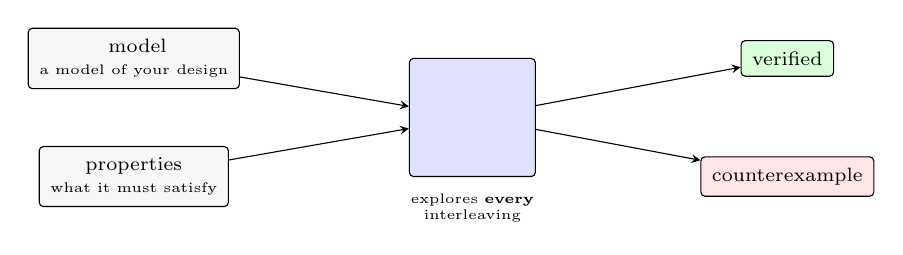
\begin{tikzpicture}[
  font=\scriptsize, >=stealth,
  b/.style={draw, rounded corners=1.5pt, align=center, inner sep=4pt,
            fill=black!3},
  lab/.style={font=\tiny, inner sep=1.5pt}
]
  \node[b] (m) at (0,0.75)  {\promelaname{} model\\{\tiny a model of your design}};
  \node[b] (p) at (0,-0.75) {properties\\{\tiny what it must satisfy}};
  \node[b, fill=blue!12, minimum height=1.5cm, minimum width=1.6cm,
        font=\small\bfseries] (s) at (4.3,0) {\spin{}};
  \node[b, fill=green!14] (ok)  at (8.3,0.75)  {verified};
  \node[b, fill=red!10]   (cex) at (8.3,-0.75) {counterexample};

  \draw[->] (m) -- (s);
  \draw[->] (p) -- (s);
  \draw[->] (s) -- (ok);
  \draw[->] (s) -- (cex);
  \node[lab, align=center] at (4.3,-1.15) {explores {\bf every}\\interleaving};
\end{tikzpicture}\par}

\vspace{0.35cm}

Either it finds no violation in {\em any} interleaving, or it hands back the one
execution that breaks the property.

\pause
\vspace{0.3cm}

\begin{itemize}
\item Developed by {\bf Gerard Holzmann}, originally at Bell Labs, later at JPL.
\item ACM {\bf Software System Award}, 2001.
\item Open source, actively used in industry and at NASA for 30+ years.
\item \url{https://spinroot.com}
\end{itemize}

\end{frame}

